We include the same systematics sources as in the 
SM Higgs analysis~\cite{HWWHCP2012} for both normalization and shapes. 
For the exotic resonance signals, such as the spin 2 
graviton ($2_\text{min}^+$), we apply additional 
shape systematics to account for the missing higher order effects. 
As discussed in Section~\ref{sec:datasel} we reweight the $m_T-m_{\ell\ell}$ templates 
derived in JHUGen-Pythia to match to the predictions by Powheg-Pythia in the SM Higgs hypothesis. 
The relative differences between the two generators in the SM Higgs case 
are then applied to the other non-SM Higgs resonances for the central shapes. 
For the non-SM Higgs hypotheses we then consider the JHUGen-Pythia 
predictions without reweighting as the $+1\sigma$ deviation from the central shape. 
The correspoinding $-1\sigma$ variation is then derived from the mirrored difference between 
the central and the $+1\sigma$ difference. 
Figure~\ref{fig:xwwshapevar} shows the central and the $\pm1\sigma$ variations 
of the $gg\to \text{Graviton}\to WW$. 

%%%%%%%%%%%%%%%%%%%%%%%%%%%%%%%%%%%%%%%%%%%%%
\begin{figure}[!hbtp]
\centering
\label{subfig:xwwshapevar}
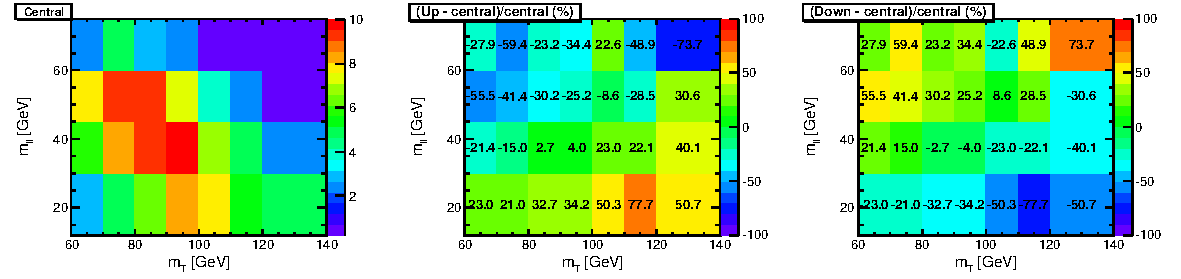
\includegraphics[width=1.05\textwidth]{figures/xww_ggHshapevar.pdf}
\caption{The shape variations for the $gg\to \text{Graviton}\to WW$. 
}
\label{fig:xwwshapevar}
\end{figure}
%%%%%%%%%%%%%%%%%%%%%%%%%%%%%%%%%%%%%%%%%%%%%
